%packages include
\documentclass[12pt, aspectratio=54, xcolor=table]{beamer}
\usepackage[utf8]{inputenc}
\usepackage{graphicx, amsmath,amsfonts,amsthm,geometry,lipsum, hyperref, caption, xcolor, animate, float}
\usepackage{hyperref, latexsym,booktabs,calligra,pstricks,stackengine, transparent, subfig}
\graphicspath{{./images/}}
\graphicspath{./animation/}
\usepackage{tikz,pgfplots, animate, listings, mathtools}
\usepackage{algorithm}
\usepackage{biblatex}
\usepackage{algpseudocode}
\usepackage{makecell}
\usepackage{color, colortbl, multirow}
\usetikzlibrary{calc, patterns, positioning}
\usetikzlibrary{shapes.geometric, arrows}

%references
\addbibresource{ref.bib}

%theme
\usepackage{custom_theme}
\setbeamertemplate{navigation symbols}{}  %hides navigation symbols
\setbeamercovered{transparent}



%for flowchart
\tikzstyle{startstop} = [rectangle, rounded corners, minimum width=2cm, minimum height=1cm,text centered, color = white, draw=white, fill=amethyst]
\tikzstyle{io} = [trapezium, trapezium left angle=70, trapezium right angle=110, minimum width=1.5cm, minimum height=1cm, text centered, color = white, draw=white, fill= atomictangerine]
\tikzstyle{process} = [rectangle, minimum width=1.5cm, minimum height=1.3cm,text centered, color = white, draw=white]
\tikzstyle{decision} = [diamond, minimum width=0.5cm, minimum height=0.5cm, text centered, color = white, draw=white, fill=asparagus]
\tikzstyle{arrow} = [thick,->,>=stealth, color = coolgrey]

%for steps
\tikzstyle{vertex} = [rectangle, rounded corners, minimum width=1cm, minimum height=1cm,text=centered,color =white, draw=white, fill=ballblue]
\tikzstyle{textonly} = [rectangle, minimum width=1cm, minimum height=0.2cm, text centered, draw=white, fill=white]
\tikzstyle{arrow1} = [ultra thick,->,>=stealth, color = lightslategray]
\tikzstyle{arrow2} = [ultra thick,->,>=stealth,dashed, color = lightslategray]


%color define
\definecolor{codegreen}{rgb}{0,0.6,0}
\definecolor{codegray}{rgb}{0.5,0.5,0.5}
\definecolor{coolgrey}{rgb}{0.55, 0.57, 0.67}
\definecolor{codepurple}{rgb}{0.58,0,0.82}
\definecolor{backcolour}{rgb}{0.95,0.95,0.92}
\definecolor{babyblue}{rgb}{0.54, 0.81, 0.94}
\definecolor{ballblue}{rgb}{0.13, 0.67, 0.8}
\definecolor{azure}{rgb}{0.0, 0.5, 1.0}
\definecolor{antiquefuchsia}{rgb}{0.57, 0.36, 0.51}
\definecolor{antiquebrass}{rgb}{0.8, 0.58, 0.46}
\definecolor{lightslategray}{rgb}{0.47, 0.53, 0.6}
\definecolor{amethyst}{rgb}{0.6, 0.4, 0.8}
\definecolor{asparagus}{rgb}{0.53, 0.66, 0.42}
\definecolor{atomictangerine}{rgb}{1.0, 0.6, 0.4}
\definecolor{brightgreen}{rgb}{0.4, 1.0, 0.4}
\definecolor{cadmiumred}{rgb}{0.89, 0.0, 0.13}
\definecolor{amber}{rgb}{1.0, 0.75, 0.0}
\definecolor{LightGreen}{rgb}{0.68,1,0.7}
\definecolor{ThemeHeader}{rgb}{0.8,0.9,1}

%for code design
\lstdefinestyle{mystyle}{
    backgroundcolor=\color{backcolour},   
    commentstyle=\color{codegreen},
    keywordstyle=\color{magenta},
    numberstyle=\tiny\color{codegray},
    stringstyle=\color{codepurple},
    basicstyle=\ttfamily\scriptsize,
    breakatwhitespace=false,         
    breaklines=true,                 
    captionpos=b,                    
    keepspaces=true,                 
    numbers=left,                    
    numbersep=5pt,                  
    showspaces=false,                
    showstringspaces=false,
    showtabs=false,                  
    tabsize=2
}

\lstset{style=mystyle}


%make title page
\title{Insertion Sort}
\subtitle{Basics, Algorithm and Program}
\author[Reyazul, Jalal, Mubasshira]{Kazi Reyazul Hasan \inst{82} \and Wasif Jalal Galib \inst{84} \and Mubasshira Musarrat \inst{88}}
\institute[BUET]{Department of Computer Science Engineering\\Bangladesh University of Engineering and Technology}
\date{\today}



\begin{document}

\begingroup
\setbeamertemplate{headline}{}
\begin{frame}
\titlepage
    \begin{figure}[htpb]
        \begin{center}
            \includegraphics[width=0.15\linewidth]{images/buet_logo1.png}
        \end{center}
    \end{figure}
\end{frame}
\endgroup


%indexpage
\begingroup
\setbeamertemplate{background} 
{
    \transparent{0.2}\includegraphics[scale = 0.255]{Algorithm.jpg}
}
\begin{frame}{Index}
\tableofcontents[sectionstyle=show,subsectionstyle=show/shaded/hide,subsubsectionstyle=show/shaded/hide]
%\onslide is useful too
\end{frame}
\endgroup


%first section
\section{Introduction}
\begin{frame}{What is Insertion Sort?}
      \textbf<1->{Insertion Sort is a type of \alert{sorting algorithm}.\\}  
      \begin{block}<2->{Sorting Alogorithm}
                A Sorting Algorithm is used to rearrange a given array or list of elements according to a comparison operator on the elements in computer language. 
      \end{block}
      \begin{example}<3->
      \begin{itemize}
          \item  Selection Sort
          \item Insertion Sort
          \item Quick Sort
          \item Merge Sort
      \end{itemize}
      \end{example}
\end{frame}

\begin{frame}[label={important}]{Sorting: Rocket Science or Human Nature?}
	\begin{figure}
		\centering
		\subfloat[\textcolor{cadmiumred}{Not Sorted}\label{fig:a}]{\includegraphics[height=4cm,width=4.5cm]{images/unsorted.jpeg}}\qquad
		\subfloat[\textcolor{codegreen}{Sorted}\label{fig:b}]{\includegraphics[height=4cm,width=4.5cm]{images/sorted.jpeg}}
		\caption*{We have been using \textbf{\alert{sorting}} for our own convenience since primitive times without really knowing or realizing any computer science documented algorithms!}
		\label{fig:1}
	\end{figure}
	
\end{frame}


\begin{frame}{Background}
\begin{structure}{\Large Historical Overview}
\vspace{14pt}
\begin{columns}

    \column<1->{0.36\textwidth}\small{Insertion Sort's real-life application ranges from sorting cards (see \ref{important}) to students' exam scripts. It might be hard to find the first person who came up with the idea behind insertion sort, because it is one of the basic ways humans would sort a list of items.}
    \column<2->{0.32\textwidth} \small{Knuth \cite{donald1999art} writes that the variant of using binary insertion was mentioned by John Mauchly as early as 1946, in the first published discussion of computer sorting, being the algorithm's first documentation.}
    \column{0.3\textwidth} 
    \begin{figure}
        \centering
         \includegraphics[scale=0.065]{images/johnmauchly.jpg}
        \caption*{\href{https://en.wikipedia.org/wiki/John_Mauchly}{John Mauchly}}
        \label{fig:2}
    \end{figure}
   
\end{columns}
\end{structure}
    
\end{frame}


%second section
%animated part
\section{Visual Representation}
\begin{frame}{Visual Representation}
\centering
\animategraphics[width=9.3cm]{14}{animation/sort-graph-}{0}{270}
\end{frame}


%
\begin{frame}{Steps in Illustration}
	\setbeamercovered{invisible}
	
	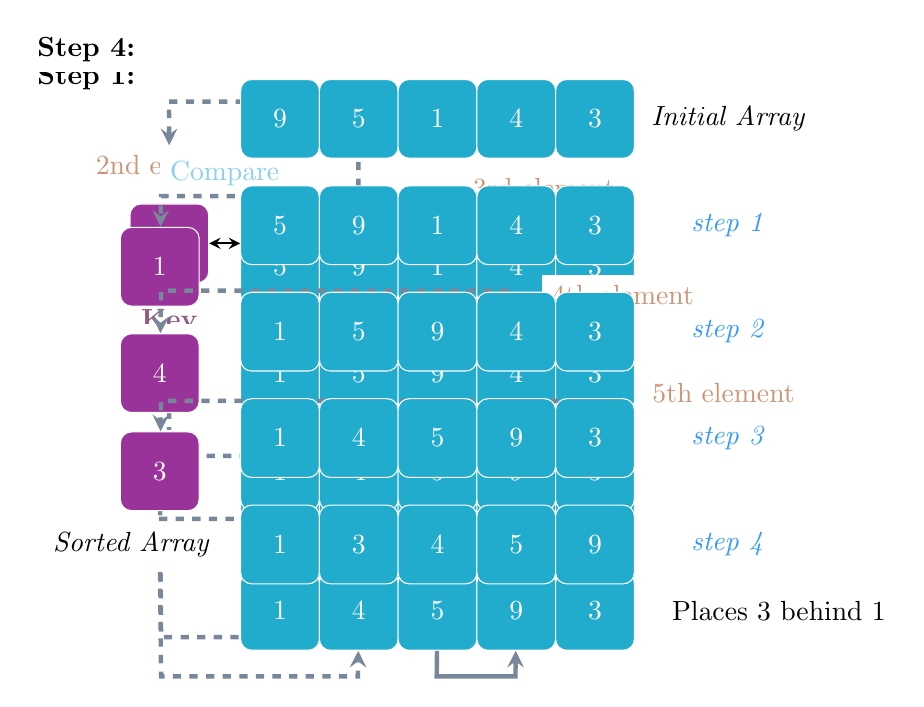
\begin{tikzpicture}
		
		\onslide<1-5>
		%row 1
		\node (1f)[vertex,xshift = 70] {9};
		\node(2f)[vertex,right of=1f]{5};
		\node(3f)[vertex,right of=2f]{1};
		\node(4f)[vertex,right of=3f]{4};
		\node(5f)[vertex,right of=4f]{3};
		
		
		\onslide<1-1>
		% initial array caption
		\node(text1)[textonly,xshift = 120, yshift = -28] {Initial Array};
		
		
		\onslide<2-5>
		%step 1
		\node(text2)[textonly,yshift=60] {\textbf{Step 1:}};
		
		
		\onslide<2-4>
		% key
		\node (key1)[vertex,fill = violet!80, xshift = 30] {5};
		\node(text3)[textonly,below of = key1] 
		{\textbf{\textcolor{antiquefuchsia}{Key}}};
		
		
		\onslide<2-2>
		% 2nd element
		\node(text4)[textonly,above of = key1]{\textcolor{antiquebrass}{2nd element}};
		%dashed arrow
		\draw[arrow2] (2f) -- (3.45, 1.8) -- (1.05, 1.8) -- (text4);
		
		
		\onslide<3-3>
		% comparison arrow
		\draw [<->,thick,>=stealth ] (1f) -- (key1);
		% comparison text
		\node[textonly, xshift = 50, yshift = 25] {\textcolor{babyblue}{Compare}};
		\node(text5)[textonly, xshift = 120, yshift = -45] {\huge $5 < 9$};
		
		
		\onslide<4-4>
		%row 2 (unsorted)
		\node (1s)[vertex,below of = 1f, yshift = -20] {9};
		\node(2s)[vertex,right of=1s]{5};
		\node(3s)[vertex,right of=2s]{1};
		\node(4s)[vertex,right of=3s]{4};
		\node(5s)[vertex,right of=4s]{3};
		% shifting arrow 9-5
		\draw[arrow1] (1s) -- (2.45, -0.8) -- (3.45, -0.8) -- (2s);
		% shifting arrow key-9
		\draw[arrow2] (text3) -- (1.05, -2.7) -- (2.45, -2.7) -- (1s);
		
		
		\onslide<5-5>
		% row 2 (sorted)
		\node (1t)[vertex,below of = 1f, yshift = -20] {5};
		\node(2t)[vertex,right of=1t]{9};
		\node(3t)[vertex,right of=2t]{1};
		\node(4t)[vertex,right of=3t]{4};
		\node(5t)[vertex,right of=4t]{3};
		\node(text6)[textonly,xshift = 125, yshift = -80] {Places 5 at the begining};
		
		
		\onslide<6->
		% row 1
		\node (1f2)[vertex,xshift = 70, yshift = 45] {9};
		\node(2f2)[vertex,right of=1f2]{5};
		\node(3f2)[vertex,right of=2f2]{1};
		\node(4f2)[vertex,right of=3f2]{4};
		\node(5f2)[vertex,right of=4f2]{3};
		
		
		\onslide<6-6>
		% step 2
		\node(text7)[textonly,yshift=70] {\textbf{Step 2:}};
		% row 2
		\node (1s2)[vertex,below of = 1f2, yshift = -25] {5};
		\node(2s2)[vertex,right of=1s2]{9};
		\node(3s2)[vertex,right of=2s2]{1};
		\node(4s2)[vertex,right of=3s2]{4};
		\node(5s2)[vertex,right of=4s2]{3};
		%key
		\node (key2)[vertex,fill = violet!80, left of = 1s2, xshift = -15] {1};
		\node(text8)[textonly,below of = key2]
		{\textbf{\textcolor{antiquefuchsia}{Key}}};
		%dashed arrow
		\draw[arrow2] (3s2) -- (4.45, 0.6) -- (0.95, 0.6) -- (key2);
		% 3rd element
		\node(text9)[textonly,above of = 4s2, xshift = 10] {\textcolor{antiquebrass}{3rd element}};
		% row 3 (unsorted)
		\node (1t2)[vertex,below of = 1s2, yshift = -25] {5};
		\node(2t2)[vertex,right of=1t2]{9};
		\node(3t2)[vertex,right of=2t2]{1};
		\node(4t2)[vertex,right of=3t2]{4};
		\node(5t2)[vertex,right of=4t2]{3};
		% shifting arrow 5-9
		\draw[arrow1] (1t2) -- (2.45, -1.3) -- (3.45, -1.3) -- (2t2);
		% shifting arrow 9-1
		\draw[arrow1] (2t2) -- (3.45, -3) -- (4.45, -3) -- (3t2);
		% shifting arrow key-9
		\draw[arrow2] (text8) -- (0.95, -3.5) -- (2.45, -3.5) -- (1t2);
		\node(text10)[textonly,xshift = 125, yshift = -120] {Places 1 at the begining};
		
		
		\onslide<7->
		% row 2
		\node (1s3)[vertex,below of = 1f2, yshift = -10] {5};
		\node(2s3)[vertex,right of=1s3]{9};
		\node(3s3)[vertex,right of=2s3]{1};
		\node(4s3)[vertex,right of=3s3]{4};
		\node(5s3)[vertex,right of=4s3]{3};
		
		
		\onslide<7-7>
		% step 3
		\node(text11)[textonly,yshift=70] {\textbf{Step 3:}};
		% row 3
		\node (1t3)[vertex,below of = 1s3, yshift = -25] {1};
		\node(2t3)[vertex,right of=1t3]{5};
		\node(3t3)[vertex,right of=2t3]{9};
		\node(4t3)[vertex,right of=3t3]{4};
		\node(5t3)[vertex,right of=4t3]{3};
		%key
		\node (key3)[vertex,fill = violet!80, left of = 1t3, xshift = -15] {4};
		\node(text12)[textonly,below of = key3]{\textcolor{antiquefuchsia}{Key}};
		%dashed arrow
		\draw[arrow2] (4t3) -- (5.45, -0.6) -- (0.95, -0.6) -- (key3);
		% 4th element
		\node(text13)[textonly,above of = 5t3, xshift = 10] {\textcolor{antiquebrass}{4th element}};
		% row 4 
		\node (1fo3)[vertex,below of = 1t3, yshift = -25] {1};
		\node(2fo3)[vertex,right of=1fo3]{5};
		\node(3fo3)[vertex,right of=2fo3]{9};
		\node(4fo3)[vertex,right of=3fo3]{4};
		\node(5fo3)[vertex,right of=4fo3]{3};
		% shifting arrow 5-9
		\draw[arrow1] (2fo3) -- (3.45, -2.5) -- (4.45, -2.5) -- (3fo3);
		% shifting arrow 9-4
		\draw[arrow1] (3fo3) -- (4.45, -4.5) -- (5.45, -4.5) -- (4fo3);
		% shifting arrow key-5
		\draw[arrow2] (text12) -- (0.95, -5) -- (3.45, -5) -- (2fo3);
		\node(text14)[textonly,xshift = 150, yshift = -140] {Places 4 behind 1};
		
		
		\onslide<8->
		% row 3
		\node (1t4)[vertex,below of = 1s3, yshift = -10] {1};
		\node(2t4)[vertex,right of=1t4]{5};
		\node(3t4)[vertex,right of=2t4]{9};
		\node(4t4)[vertex,right of=3t4]{4};
		\node(5t4)[vertex,right of=4t4]{3};
		
		
		\onslide<8-8>
		% step 4
		\node(text15)[textonly,yshift=70] {\textbf{Step 4:}};
		%row 4(unsorted)
		\node (1fo4)[vertex,below of = 1t4, yshift = -22] {1};
		\node(2fo4)[vertex,right of=1fo4]{4};
		\node(3fo4)[vertex,right of=2fo4]{5};
		\node(4fo4)[vertex,right of=3fo4]{9};
		\node(5fo4)[vertex,right of=4fo4]{3};
		%key
		\node (key4)[vertex,fill = violet!80, left of = 1fo4, xshift = -15] {3};
		\node(text16)[textonly,below of = key4]{\textcolor{antiquefuchsia}{Key}};
		%dashed arrow
		\draw[arrow2] (5fo4) -- (6.45, -2) -- (0.95, -2) -- (key4);
		% 5th element
		\node(text17)[textonly,above of = 5fo4, right of =5fo4,xshift = 18] {\textcolor{antiquebrass}{5th element}};
		%row 5
		\node (1fi4)[vertex,below of = 1fo4, yshift = -22] {1};
		\node(2fi4)[vertex,right of=1fi4]{4};
		\node(3fi4)[vertex,right of=2fi4]{5};
		\node(4fi4)[vertex,right of=3fi4]{9};
		\node(5fi4)[vertex,right of=4fi4]{3};
		% shifting arrow 4-5
		\draw[arrow1] (2fi4) -- (3.45, -3.7) -- (4.45, -3.7) -- (3fi4);
		% shifting arrow 5-9
		\draw[arrow1] (3fi4) -- (4.45, -5.5) -- (5.45, -5.5) -- (4fi4);
		% shifting arrow 9-3
		\draw[arrow1] (4fi4) -- (5.45, -3.7) -- (6.45, -3.7) -- (5fi4);
		% shifting arrow key-4
		\draw[arrow2] (text16) -- (0.95, -5.5) -- (3.45, -5.5) -- (2fi4);
		\node(text18)[textonly,right of = 5fi4, xshift = 38] {Places 3 behind 1};
		
		
		\onslide<9->
		%row 4(unsorted)
		\node (1fo5)[vertex,below of = 1t4, yshift = -10] {1};
		\node(2fo5)[vertex,right of=1fo5]{4};
		\node(3fo5)[vertex,right of=2fo5]{5};
		\node(4fo5)[vertex,right of=3fo5]{9};
		\node(5fo5)[vertex,right of=4fo5]{3};
		%row 5(sorted)
		\node (1fi5)[vertex,below of = 1fo5, yshift = -10] {1};
		\node(2fi5)[vertex,right of=1fi5]{3};
		\node(3fi5)[vertex,right of=2fi5]{4};
		\node(4fi5)[vertex,right of=3fi5]{5};
		\node(5fi5)[vertex,right of=4fi5]{9};
		%texts
		\node(text20)[textonly,right of = 5f2, xshift = 20]{\textit{Initial Array}};
		\node(text20)[textonly,right of = 5s3, xshift = 20]{\textcolor{azure!80}{\textit{step 1}}};
		\node(text20)[textonly,right of = 5t4, xshift = 20]{\textcolor{azure!80}{\textit{step 2}}};
		\node(text20)[textonly,right of = 5fo5, xshift = 20]{\textcolor{azure!80}{\textit{step 3}}};
		\node(text20)[textonly,right of = 5fi5, xshift = 20]{\textcolor{azure!80}{\textit{step 4}}};
		\node(text20)[textonly,left of = 1fi5, xshift = -25]{\textit{Sorted Array}};
		
		
	\end{tikzpicture}
	
	
\end{frame}


\begin{frame}{Flowchart}

	\scriptsize{
		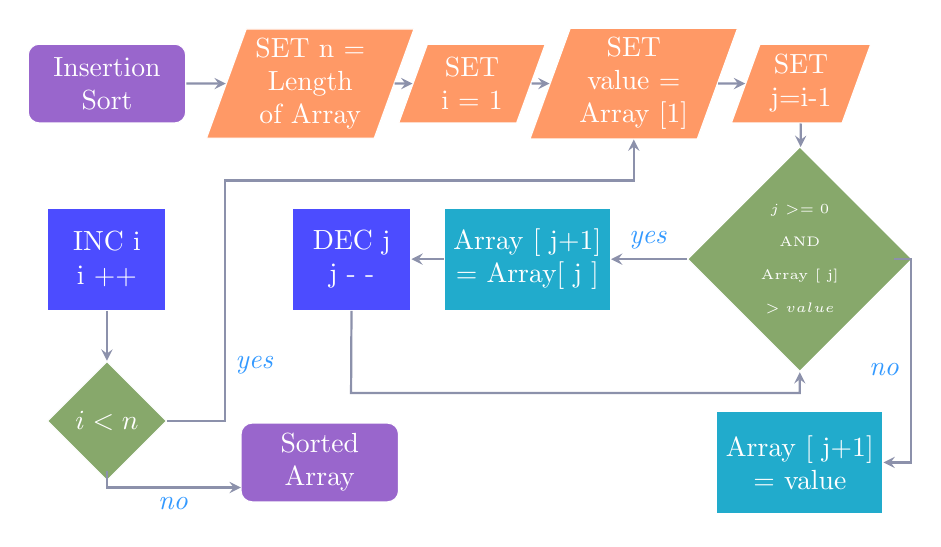
\begin{tikzpicture}[every text node part/.style={align=center}]
			
			% row 2
			\node (1) [process,fill=blue!70] {INC i \\ i ++};
			\node (2) [process,fill=blue!70, right of = 1, xshift = 60] {DEC j \\ j - -};
			\node (3) [process,fill=ballblue, right of = 2, xshift = 35] {Array [ j+1] \\= Array[ j ]};
			\node (4) [decision, right of = 3, xshift = 70] {\tiny{$j >= 0$} \\ \tiny{AND} \\ \tiny{Array [ j]} \\ \tiny{$ > value$}} ;
			
			% row 1
			\node (start) [startstop, above of = 1, yshift = 35] {Insertion \\Sort};
			\node (5) [io, right of = start, xshift = 45] {SET n = \\ Length \\ of Array};
			\node (6) [io, right of = 5, xshift = 30] {SET  \\ i = 1};
			\node (7) [io, right of = 6, xshift = 30] {SET  \\ value =\\ Array [1]};
			\node (8) [io, right of = 7, xshift = 32] {SET  \\ j=i-1};
			
			% row 3
			\node (9) [process,fill=ballblue, below of = 4, yshift = -45] {Array [ j+1] \\= value};
			\node (10) [decision, below of = 1, yshift = -30] {$i<n$};
			\node (stop) [startstop, left of = 9, xshift = - 145] {Sorted \\Array};
			
			%arrows
			\draw [arrow] (start) -- (5);
			\draw [arrow] (5) -- (6);
			\draw [arrow] (6) -- (7);
			\draw [arrow] (7) -- (8);
			\draw [arrow] (8) -- (4);
			\draw [arrow] (4) -- node[anchor=south] {\textcolor{azure!80}{\textit{yes}}}(3);
			\draw[arrow] (3) -- (2);
			\draw[arrow] (2) --(3.1,-1.7) -| (4);
			\draw[arrow] (10,0) -- (10.21,0) node[anchor=east,yshift = -40] {\textcolor{azure!80}{\textit{no}}} |- (9);
			\draw[arrow] (1) -- (10);
			\draw[arrow] (10) -|node[anchor=west, yshift = 20] {\textcolor{azure!80}{\textit{yes}}}(1.5,1)-| (7);
			\draw[arrow] (0, -2.69) -- (0,-2.9) -- node[anchor=north] {\textcolor{azure!80}{\textit{no}}}(1.7,-2.9);
			
			
	\end{tikzpicture} } 
\end{frame}

\section {Implementation}
\subsection{Algorithm}
\begin{frame}[fragile]{Algorithm}
    
\begin{algorithm}[H]
\caption{Insertion algorithm}\label{insertion}
\begin{algorithmic}[1]
\Procedure{insertionSort}{$A: array$}
\State $n\gets length(A)$
\For{\texttt{i:=1 to n-1}}
\State $j\gets i$
\While{\texttt{j > 0 and A[j-1] > A[j]}}
\State{\texttt{swap(A[j], A[j-1])}}
\State $j\gets j-1$
\EndWhile\label{endwhile} \Comment{inner loop end}
\EndFor\Comment{outer loop end}
\EndProcedure
\end{algorithmic}
\end{algorithm}

\end{frame}

    


\subsection{Code}

\begin{frame}[fragile]{Complete Program in Python}
    \tiny{
    \begin{lstlisting}[language=Python]
# Insertion sort in Python
def insertionSort(array):

    for step in range(1, len(array)):
        key = array[step]
        j = step - 1
        
        # Compare key with each element on the left of it until an element smaller than it is found      
        while j >= 0 and key < array[j]:
            array[j + 1] = array[j]
            j = j - 1
        
        # Place key after the element just smaller than it
        array[j + 1] = key

data = [9, 5, 1, 4, 3]
insertionSort(data)
print('Sorted Array in Ascending Order:')
print(data)   \end{lstlisting}
   }
\textit{See \cite{Code}}
\end{frame}

\section{Analysis}
\begin{frame}{Best Case}
The \textcolor{codegreen}{best case} of Insertion Sort occurs \textbf{if the array is already sorted.} When $j=i-1$, we always find the key $A[i]$ the first time.\\
Therefore, the running time of an algorithm equation-
\begin{equation*}
	\begin{multlined}
	T(n)= c_1n+c_2(n-1)+c_4(n-1)+c_5\sum_{2\leq j\leq n}^{}(1) \\ +c_6\sum_{2\leq n}^{}(1-1)+c_7\sum_{2\leq n}^{}(1-1)+c_8(n-1)
		\end{multlined}
\end{equation*}
simplifies as,\\
\begin{equation*}
	T(n)= an+b= 
	\mathcal{O}(n)
\end{equation*}
	
    
\end{frame}

\begin{frame}{Worst Case}
	The \textcolor{cadmiumred}{worst case} occurs \textbf{if the array is in reverse order of how we need to sort it.} So, we must compare each element $A[j]$ with element in the entire sorted subarray $A[i .. j-1]$.\\
	The running term hence simplifies as,
	\begin{equation*}
		T(n)= an^2+bn+c= 
		\mathcal{O}(n^2)
	\end{equation*}
Since we focus more on worst case, the complexity of insertion sort is said to be \textbf{\textit{$n^2$}}.
\end{frame}

\begin{frame}{Complexity Increase by Element}
	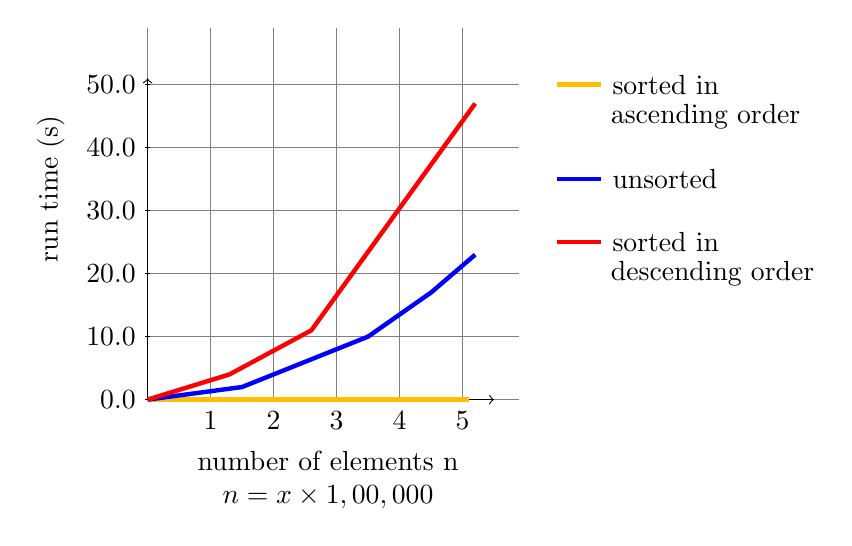
\begin{tikzpicture}[every text node part/.style={align=center},scale = 0.8]
		
		\draw[step=1cm,gray,very thin] (0,0) grid(5.9,5.9);
		\draw[->] (0,0) -- (5.5,0) node[anchor=north , xshift = -60, yshift = -15] {number of elements n \\ $n = x \times 1,00,000$};
		\draw[->] (0,0) -- (0,5.1) node[anchor=east, rotate = 90, yshift = 35, xshift =-10] {run time (s)};
		\foreach \x in {1,2,3,4,5}
		\draw (\x cm,1pt) -- (\x cm,-1pt) node[anchor=north] {$\x$};
		\foreach \y in {0,1,2,3,4,5}
		\draw (1pt,\y cm) -- (-1pt,\y cm) node[anchor=east] {\pgfmathparse{\y * 10}\pgfmathresult};
		\draw[ultra thick,amber] (0,0) -- (5.1,0);
		\draw[ultra thick,blue] (0,0) -- (1.5, 0.2) -- (2.5, 0.6) --(3.5, 1) -- (4.5,1.7) -- (5.2, 2.3);
		\draw[ultra thick,red] (0,0) -- (1.3, 0.4) -- (2.6, 1.1) -- (5.2, 4.7);
		
		\draw[ultra thick, amber] (6.5,5) -- (7.2,5) node [anchor = west]{\textcolor{black}{sorted in}};
		\draw[white] (6.5,4.5) -- (7.2,4.5) node [anchor = west]{\textcolor{black}{ascending order}};
		\draw[ultra thick, blue] (6.5,3.5) -- (7.2,3.5) node [anchor = west]{\textcolor{black}{unsorted}};
		\draw[ultra thick, red] (6.5,2.5) -- (7.2,2.5) node [anchor = west]{\textcolor{black}{sorted in}};
		\draw[white] (6.5,2) -- (7.2,2) node [anchor = west]{\textcolor{black}{descending order}};
	\end{tikzpicture} 
	
\end{frame}

\begin{frame}{Complexity Overview}
We can compare different sorting algorithm complexities with insertion sort from the given table.
\begin{table}

	\resizebox{\linewidth}{!}{
		\bgroup
		\def\arraystretch{1.5}%  1 is the default, change whatever you need

		\begin{tabular}{c|c|c|c|c}
			\Xhline{5\arrayrulewidth}
			%\rowcolor{ThemeHeader}
			& \multicolumn{3}{|c|}{\textbf{Time Complexity}} & \textbf{Space Complexity} \\
			\cline{2-5}
			%\rowcolor{ThemeHeader}
			\multirow{-2}{*}{\textbf{Sorting Algorithm}} & \textbf{Best Case} & \textbf{Average Case} & \textbf{Worst Case} & \textbf{Worst Case} \\
			\Xhline{5\arrayrulewidth}
			Bubble Sort & $\Omega(N)$ & $\Theta(N^2)$ & $O(N^2)$ & $O(1)$ \\
			\Xhline{0.5pt}
			Selection Sort & $\Omega(N^2)$ & $\Theta(N^2)$ & $O(N^2)$ & $O(1)$ \\
			\Xhline{0.5pt}
			\rowcolor{LightGreen}
			Insertion Sort & $\Omega(N)$ & $\Theta(N^2)$ & $O(N^2)$ & $O(1)$ \\
			\Xhline{0.5pt}
			Quick Sort & $\Omega(N log_2 N)$ & $\Theta(N log_2 N)$ & $O(N^2)$ & $O(N)$ \\        
			\Xhline{0.5pt}
			Merge Sort & $\Omega(N log_2 N)$ & $\Theta(N log_2 N)$ & $O(N log_2 N)$ & $O(N)$ \\
			\Xhline{0.5pt}
			Heap Sort & $\Omega(N log_2 N)$ & $\Theta(N log_2 N)$ & $O(N log_2 N)$ & $O(1)$ \\
			\Xhline{5\arrayrulewidth}
	\end{tabular}


	\egroup}
		\caption*{\scriptsize{Time and Space Complexity of Sorting Algorithms}}
\end{table}
	
\end{frame}




\begin{frame}{References}
   \printbibliography 
\end{frame}

\end{document}
